
\section{Verification method}
\label{alg1}
As a result of lemma \ref{lemma1}, if $\gamma_k^{k+1} \cap Bad$ = $\empty$ for any \e{k} $\geq$ 1, then $\gamma_k(V) \cap Bad$ = $\empty$ for any buffer size larger than \e{k}. Given a set of bad states \e{Bad}, a set of initial states \e{I} and a set of transitions, Verifying the correctness of a system can be done with the following algorithm.

\begin{algorithm}
  \caption{General Verification algorithm}\label{euclid}
  \begin{algorithmic}[1]
      \For{\texttt{$True$}}
        \If {$\mathcal{R}_k$ $\cap$ $Bad$ $\neq$ $\emptyset$} 
        \State return Unsafe
        \EndIf
        \State V := $\mu X.\alpha_k(I)$ $\cup$ $Apost_k(X)$
        \If {$\gamma_k(V)$ $\cap$ $Bad$ = $\emptyset$} 
        \State return Safe     
        \EndIf
        \State k := k+1
      \EndFor
\end{algorithmic}
\end{algorithm}

The algorithm begins by performing a reachability analysis in order to compute $\mathcal{R}_k$ and check for bad states. For any buffer size \e{k}, if a bad state is found to be reachable in $\mathcal{R}_k$, the system is unsafe and the algorithm terminates. If no such bad state was found, the algorithm continues by computing an \e{overapproximation} of configurations of size $k$, reachable through configurations of size at most $k+1$ and checking for bad configurations. This is done by computing $Apost_k$ iteratively until a fixpoint \e{V} is reached. If at this point no bad configuration has been found, the system can be said to be safe (due to the result of \ref{lemma1}) and the algorithm terminates. If on the other hand a bad state was found, the system is not necessarily unsafe, as \e{V} is an over-approximation of the reachable states in $\mathcal{R}_k$, the process is repeated with a buffer size of \e{k+1}.

In this rest of this section, we show how to implement this algorithm in an efficient way. We do this by beginning with a naive algorithm computing the configurations, and then step by step locating and addressing the performance issues. 

\todo{Is the algorithm guaranteed to terminate? When does it not?}


\subsection{Naive algorithm}
A naive way to generate configurations would be to perform the described operations such that they correspond directly to the mathematical notations as described in section \ref{alphagamma}. This is possible, as most programming languages have built-in datastructures that support set operations.

A transition in the transition system corresponds to one or more \e{rules} in the implementation. A rule \e{r} $\in$ \e{R} is a description of a transition, seen as a set of state-predicates, channel-predicates, state-effects and channel-effects.If all predicates are true for a configuration \e{c}, the effects of the rule are applied to \e{c} resulting in a post-value \e{c'}.

In this naive approach, all configurations are stored in a \e{set}, such that each configuration is stored uniquely. For each element \e{c} of the set \e{V}, the function \e{gamma}, \e{step} and \e{alpha} are performed in order, until a \e{fix-point} is reached, i.e. continuing the process does not result in any more configurations being found. Assuming that a set of channel symbols and a set of rules \e{R} describing the transitions are known, the algorithm does the following:

\begin{enumerate}
\item
Generate a set $\Gamma(V)$: For each configurations \e{c} $\in$ \e{V}, generate all potential concretizations \e{con} such that \e{|con|} = \e{|c|}+1. For any such potential concretization \e{con}, remove those for which $alpha_k(c')$ $\not\subset$ $V$.

\item
Generate the $post(V)$: For every \e{con} $\in$ $\Gamma(V)$, \e{r} $\in$ \e{R}, compute \e{r(con)}.

\item
Generate Apost(V): For each element \e{p} $\in$ \e{post(V)}, compute its views of size \e{k}. If \e{V'} $\cup$ \e{V} = \e{V}, a fixpoint has been reached, otherwise the processes repeats with \e{V} := \e{V} $\cup$ \e{V'}.
\end{enumerate}

The bottle-neck in this algorithm lies in \e{gamma}. It first creates all potential concretizations of a configuration \e{c}, i.e. all combinations of channel evaluations where at least one of the channels is of a larger size than in \e{c}. Additionaly, for each of these, all their views must be computed in order to determine whether the concretization should be refuted or not. Although this method is correct, there is significant overlap of concretizations; it is often possible to create the same concretization \e{con} in several ways, and each time, $\alpha_k{con}$, \e{post(con)} and \e{Apost(con)} need be performed. In the next section, we show abstractions of the functions \e{alpha} and \e{gamma} that are less computationally expensive.


\subsection{Solution}
We look closer at $\gamma$, in order to address the issues mentioned above. We show that all concretizations can be found, while considering only a subset of the potential concretizations. Furthermore, it is possible to determine whether a concretization should be accepted or not, examining only a subset of its views. 

\paragraph{Abstracting the concretizations.}
Given a configuration \e{c}, with channel evaluations $\xi$ such that all channels have size smaller or equal to \e{k}, a potential concretization of \e{c} is any configuration \e{con} such that \e{con} can be created from \e{c} by appending a symbol to at least one of the channels of \e{c}. As this is a large number of potential configurations, it is desireable to consider only a subset thereof, while still ensuring that all valid concretizations are eventually found.

We show that it is sufficient to in each iteration consider only the potential concretizations of \e{c}, for which only one channel has been modified, and only modifications where a symbol has been added at the \textbf{end} (or alternatively the beginning) of a channel.

Consider a potential concretization \e{con} of \e{c}, where $n$ channels have been extended by a symbol. If such a potential concretization is valid, any evaluation where $n'<n$ channels have been modified in a similar way will also be a valid concretization. Therefore, \e{con} will eventually be considered also when only one channel is extended in each iteration, but more iterations are required in order to find it.

As an example, consider a concretization with channel evaluation \e{e} = $w_1..w_l$, created by extending some configuration with a single symbol, not necessarily at the end of the channel. If \e{con} is a valid concretization, then a configuration \e{c'} must be in \e{V} such that \e{c'} has the channel evaluation $w_1..w_{l-1}$, since \e{c'} $\in$ $\alpha_k(con)$. This channel evaluation can be extended to \e{con} by adding the symbol $w_l$ at the end of the channel.

This shows that any valid concretization will eventually be created, even if only a subset of potential concretizations are created in each iteration. This result highly reduces the number of potential concretizations inspected. If \e{s} = |$symbols$|, \e{t} is the number of channels and \e{n} = |$V$|, the naive method creates $O(n*(s^k)^t)$ potential concretizations in each iteration. Using this abstraction, the number of potential concretizations is reduced to $O(n*s*t)$.

\paragraph{Reducing the views.}
Suppose we want to determine whether \e{c} $\in$ $\gamma_k(V)$ given a configuration \e{c} and a set \e{V}. This would require that all views \e{v} $\in$ $\alpha_k(c)$ are in \e{V}. Consider a view \e{v} = $\conf{S, \xi(ch)=w}$ with size($w$) = $k$; if \e{v} $\in$ \e{V} then necessarily, any \e{v'} = $\conf{S, \xi(ch)=w'}$ with \e{w'} $\sqsubseteq$ \e{w} $\in$ \e{V}. Consequently, it is sufficient to assure that all configurations \e{c} = $\conf{S,\xi(ch_i)=w_i}$ are in \e{V}, with

\begin{itemize}
\item
size($w_i$)=$k$ if size($\xi(ch)$) $\geq$ $k$
\item
size($w_i$)= size($\xi(ch)$) if size($\xi(ch)$) < $k$.
\end{itemize}

\subparagraph{Example.} Suppose we want to determine whether the potential concretization \e{con} = $\conf{S, abc, de}$ is an element of $\gamma_2$. It is then sufficient to check that $c_1$ = $\conf{S,ab,de}$ and $c_2$ = $\conf{S,bc ,de}$ are in \e{V}. The potential concretization must have been created from either $c1$ or $c_2$. Because of this, it is always sufficient to check for the existence of a single configuration, to determine wether \e{con} should be accepted.
\\\\

Using these abstraction, the computational complexity of the verifier is greatly reduced, but there are yet several ways to optimize the procedure. The bottle-neck with the procedure at its current state is the choice of a \e{Set} as lone data structure to store configurations. We expect the number of configurations to grow rather large, due to state-space explotion which cannot be avoided automatically (in certain cases, it could be reduced by further abstraction of the model under testing or by removing unnecessary redundancy in the model). Assuming the Set is ordered, inserting an element to the set and finding an element in the set is done in \e{O(log n)} where \e{n} is the number of elements in the set. As a consequence, the function \e{alpha} which determines whether the views of a certain configuration are in the set has complexity $O(p \cdot log n)$ where \e{p} = $|\alpha_k(c)$. We observe that by definition, a view (and a configuration) is of type \e{(S $\times$ $\xi$)}. For any configuration \e{c} = $\conf{s}{\xi}$, it's views will be of the type $\conf{s}{\xi'}$, i.e., the configuration and its views have identical control-parts. It is therefore reasonable to divide the single \e{Set} into a Set of \e{Set}s, where each \e{Set} corresponds to a specific control-state. With such a division, it is sufficient to check whether the views of a configuration reside in the \e{Set} that corresponds to its control-state.

In a best-case scenario, there would be an equal number of configurations for every state in the system. The complexity of checking whether $\alpha_k(c)$ $\in$ $V$ is reduced to $O(p \cdot log (n/s))$ where \e{s} denotes the number of states in the system. The gains of these modifications in terms of computational complexity is difficult to determine, as the number of configurations with a certain control-state are not necessarily well-distributed, but we anticipate that the gains in many cases will be close to the best case scenario.

% Det går inte att beskriva rule-delen här, för det är mer beroende av tries.
\subsection{Even less naive algorithm}
\subsubsection{Control-State Partitioning}
Above it was suggested that the set V could be divided into several sets, distinguished by control-states. The number of control-states in a system is finite and unique; For a system with \e{n} processes, the number of states is $\prod\limits_{i=1}^n|p_i|$. This makes it possible to partition the set of configurations into several smaller disjoint sets, such that all configurations in a set have equal control-state. These sets can be stored in a hashmap indexed by control-state. 

%\begin{figure}
%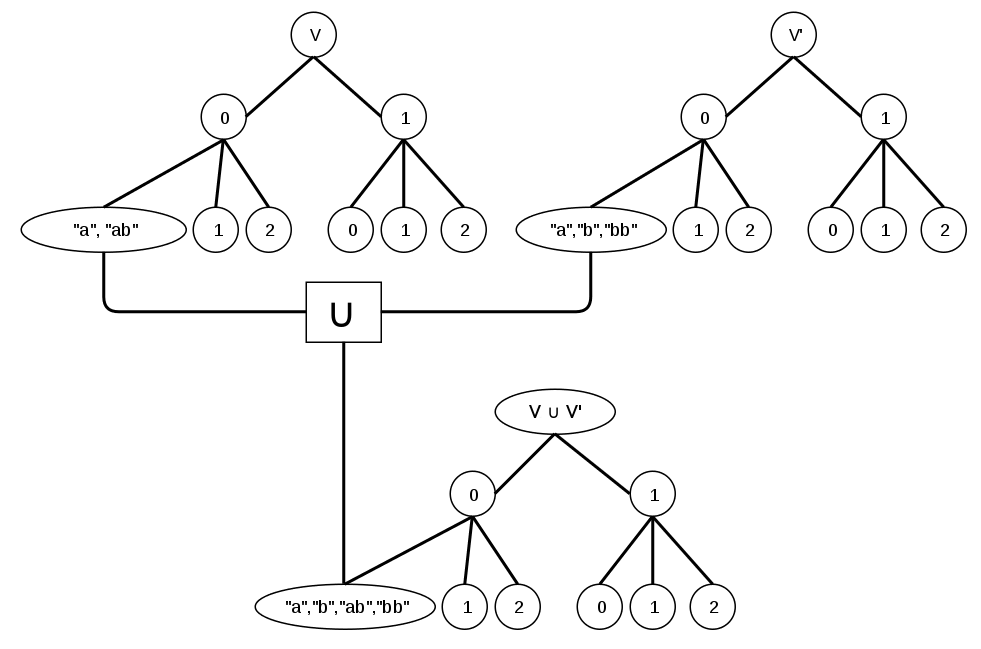
\includegraphics[width=400pt] {bilder/triemerge.png}
%\caption{This picture shows the union of two tries. In this case, there are two processes, the first of which has two states (0 and 1) and the second has three states (0,1 and 2). The union of the trie is the union of their leaves. In the picture, the content of the leaves (0,0) in both threes is made explicit.}
%\label{triemerge}
%\end{figure}


\subsubsection{Advantages of Partitioning}
Using this partitioning, each node in the hashmap is a \e{Set} with equal-state configurations, addressed by the common control-state. Compared to the previous solution, this leads to a speed-up when inserting, retrieving and looking for the existence of elements in the sets, as the size of the sets will be smaller than before. Retrieving and inserting nodes into the hashmap is done in constant time in practice (the number of elements will be static, avoiding the need of resizing the hashmap).

Having partitioned the configurations, consider the act of applying a rule in order to create a new configuration. Recall that any rule has a state-predicate, a channel-predicate, a state-event and a channel-event. If the predicates are fulfilled, a new configuration can be created by applying the events to the current configuration.

By organizing the set of \e{rules} or transitions in a similar way in a hashmap of rules, we can ensure that the state-predicate is fulfilled without specifically testing for it. A state-predicate is a (possible empty) predicate on the states of the processes in the system, requiring that one or more processes are in a specific state. It is therefore possible to generate a static hashmap of rules, addressed again by control-states.

Considering a transition $t_2$ with no requirements on any processes, the state-predicate will be fulfilled by any configuration, thus a corresponding rule is created in every node of the tree. Consider then instead a transition $t_2$ with requirements on all the processes in the system, i.e. there is only one valid control-state. Such a transition corresponds to a single rule in the node addressed by that control-state. Last, consider a transition $t_3$ with requirements on a true subset of the processes in the system, then the transition can be taken from a number of control-states. These control states can be generated, and the transition will correspond to a set of rules in the nodes corresponding to those control-states.

\paragraph{Example.} Consider yet again the alternating bit protocol, as described in \ref{REFERERA DEN MED OBSERVER}. The system has three processes \e{Sender}, \e{Receiver} and \e{Observer} with 4, 4 and 3 states respectively. Consider then the transition with the predicates that the sender is in state 3, the observer in state 3 and they may take the synchronized transition with the action \e{Snd} to states 4 and 2 respectively. This transition has no requirements on the receiver, thus it corresponds to four rules, (3,1,3)->(4,1,2), (3,2,3)->(4,2,2), (3,3,3)->(4,3,2), (3,4,3)->(4,4,2). These rules are inserted in the nodes (3,1,3), (3,2,3), (3,3,3) and (3,4,3).

There is a small one-time cost of creating the rule tree, but after creation, it is highly effective. The division by itself ensures that the state-predicate is fulfilled, if not, we never even attempt to apply the rule to a configuration. We illustrate this in figure \ref{applyrule} 

\begin{figure}
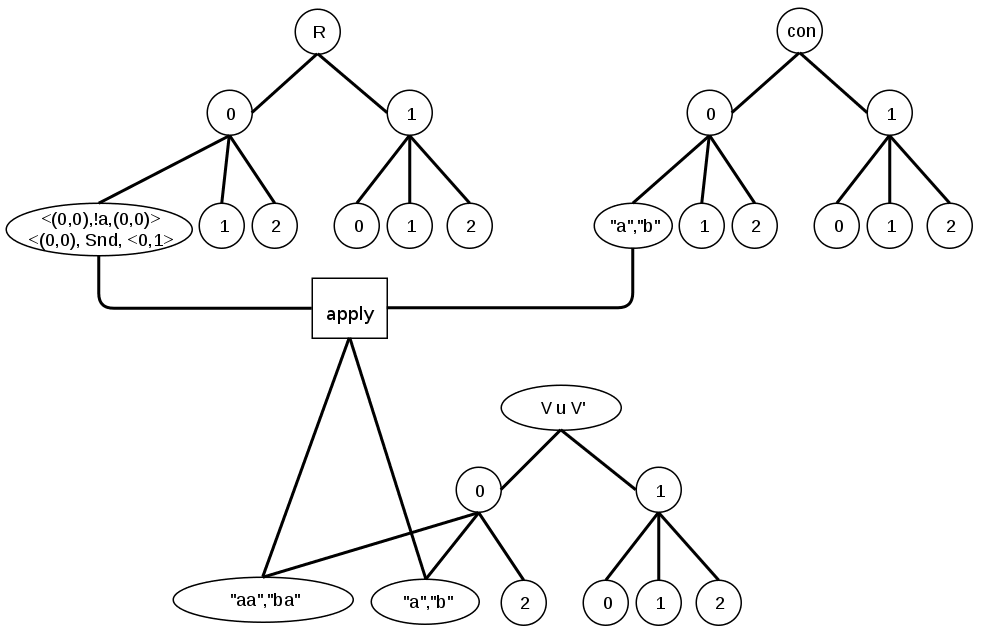
\includegraphics[width=400pt] {bilder/applyrule.png}
\caption{This picture shows the process of applying rules. For each control-state, each rules with that state are applied on each configuration with the same state. This will generate new configurations, not necessarily with the same control-state. This is visualized in a tree, rather than a hashmap, only since hashmap are less intuitive to draw.}
\label{applyrule}
\end{figure}


\begin{algorithm}
  \caption{The verification algorithm from section \ref{alg1} in somewhat higher detail. This version includes }\label{euclid}
  \begin{algorithmic}[1]
    \State \textbf{Gamma (V, Seen):}
    \State \hspace{6 mm} con' := concretizations (V)
    \State \hspace{6 mm} con  := c | c $\in$ con $\land$ c $\notin$ Seen
    \\
    \State \textbf{Step (Con, Rules):}
    \For {state $\in$ nodes(V)}
    \State \hspace{6 mm} S := r(c) | $\forall$ c $\in$ con(state) $\land$ $\forall$ r $\in$ Rules(state)
    \EndFor
    \\            
    \State \textbf{Alpha (V, S):}
    \State \hspace{6 mm} V:= V $\cup$ views(C)
    \\
    \State \textbf{Verifier (V, Rules, Bad):}
    \For{\texttt{$True$}}
        \If {$\mathcal{R}_k$ $\cap$ $Bad$ $\neq$ $\emptyset$} 
        \State return Unsafe
        \EndIf
        \State V := $\mu Alpha(Step(Gamma(V)))$
        \If {$\gamma_k(V)$ $\cap$ $Bad$ = $\emptyset$} 
        \State return Safe     
        \EndIf
        \State k := k+1
      \EndFor
\end{algorithmic}
\end{algorithm}


\subsection{Final subsection}
An efficient algorithm in this context is largely an algorithm that avoids performing unnecessary calculations. This can either be done by avoiding to create unnecessary configurations such as was done with the rule hashmap above or by avoiding re-calculating previously calculated results. The algorithm as described above reproduces its steps each iteration; if a configuration \e{c} can be extended to a concretization \e{con} at any point in the verification process, then \e{con} can and will be created in every following iteration. This includes checking whether \e{$\alpha_k(con) \subset V$}, applying a set of rules to the configuration and then adding all the views of the resulting configurations to the set. Each time the calculations are performed, the result will be duplicates and no new views are added to the system.

We solve this by maintaining another hashmap, \e{seen}, of configurations in parallell, containing exactly those concretization that have been accepted. If a configuration \e{c} can be extended to the concretization \e{con}, then we first check if \e{con} is an element of seen. If it is, we discard \e{con}, otherwise we add \e{con} to \e{seen} and also to the set of concretizations to be evaluated in this iteration.

Yet another source of repetition is the fact that there are multiple ways to create the same channel evaluations. Therefore, after a rule has been applied to a concretization, it may result in a configuration already in the set. Instead of performing the costly $\alpha$-calculation, we first check if the newly created configuration is not in fact a duplicate by checking if it is already in \e{V}. If so, the configuration can again be discarded.

The final algorithm amounts to the following pseudo-code representation:

\subsection{Reachability Analysis}
An intricate part of the verification process is to perform a reachability analaysis, looking for bad states. 
\todo{Wouldn't this be the same as the algorithm above, but without the creation of concretizations and not alloweing words larger than k??? I could re-use all code}.

\subparagraph{Finding Minimal Traces}
When running the verification, if a bad state is found we want to produce a trace leading up to the bad state. Preferably, this would be a minimal trace that leads to the bad state.
 
The proposed verification method generates a finite set of reachable states (nodes in this context), but it does not record the available transitions between the nodes (i.e. the edges). It is possible to for each node \e{n} to save all nodes \e{n} from which an edge to \e{n'} exists, and thus build the complete reachability graph of the problem. There exists efficient algorithms to solve such a problem, e.g. \e{dijkstra shortest path}, or even the shortest path between any two nodes, e.g. flow-network techniques. Although these algorithms are efficient, building the complete reachability graph would be costly in terms of memory space, as the number of edges may be much larger than the number of states.

 
We show that due to the method of iteratively constructing the graph, nodes are created in such a way, that if a node $n_{i}$ created in the \e{i}:th iteration is reached by a node $n_{i-1}$ over an edge $e_{i-1}$, the shortest path from the initial node $n_0$ will necessarily be a path $e_1...e_{i-1}$.
 
\e{Proof.} This is proven using an induction proof. We hypothesize that, if at the point of creation of $n_i$, choosing the parent node $n_{i-1}$ from which an edge $e_{i-1}$ can be taken $n_i$, the path $e_1..e_{i}$ will be the shortest path to $n_i$ and has length \e{i}. Note that the node $n_{i-1}$ must have been created in the previous iteration; had it been created earlier, the edge $e_i$ could have been taken in a previous iteration, and so $n_{i+1}$ would already be a node in the tree.
 
The base case is that for any node reachable from $n_0$ over any edge $e_0$, $e_0$ will be the shortest path and has length 1. This is trivially true.
 
Now suppose a node $n_{i+1}$ is reachable over an edge $e_i$ from a node $n_i$, and the node $n_{i+1}$ is not yet in the system. The induction hypothesis states that the path $e_1...e_i$ is the shortest path leading up to $n_i$. If $e_0..e_{i-1}e_i$ would not be the shortest path to $n_{i+1}$, there would be a path $e'_0..e'_{k-1}$ to another node $n_k$ with k < i from which $n_{i+1}$ can be reached. But any such node would have been created in the \e{k}:th iteration of the algorithm, which would contradict the fact that the node $n_{i+1}$ was not already in the system.
 
Having shown this, we need only record the information of a single parent of a node, in order to build up a tree from which the shortest path from $n_0$ to any node in the system can efficiently be found.


\swreceiver

\swobserver

\swsender
